
% These lines tell TeXShop to typeset with xelatex, and to open 
% and save the source with Unicode encoding.

%!TEX TS-program = xelatex
%!TEX encoding = UTF-8 Unicode

\documentclass[12pt]{article}
\usepackage{geometry}  
\geometry{letterpaper}   
\usepackage{graphicx}
\usepackage{amssymb}

% Will Robertson's fontspec.sty can be used to simplify font choices.
% To experiment, open /Applications/Font Book to examine the fonts 
% provided on Mac OS X, and change "Zapfino" to any of these choices.

\usepackage{fontspec,xltxtra,xunicode}
\defaultfontfeatures{Mapping=tex-text}
\setromanfont[Mapping=tex-text]{Zapfino}
\setsansfont[Scale=MatchLowercase,Mapping=tex-text]{Gill Sans}
\setmonofont[Scale=MatchLowercase]{Andale Mono}

\title{Brief Article}
\author{The Author}

\begin{document}
\maketitle

This is a standard \TeX\ document using Zapfino type. It uses \LaTeX\ and
the standard \TeX\ graphic packages.

\begin{figure}[htbp] 
   \centering
   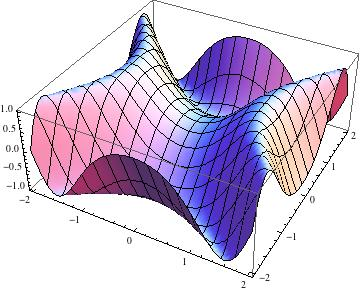
\includegraphics[width=2in]{XeTeX-2.jpg} 
   \caption{from Mathematica}
\end{figure}

\end{document}  